\documentclass[12pt,letterpaper]{article}
\usepackage{pdfpages}
\usepackage{fancyhdr}
\usepackage[colorlinks=true, urlcolor=blue, linkcolor=blue]{hyperref}
\usepackage{graphicx}
\usepackage[top=1.4in, left=0.5in, right=0.5in, bottom=0.8in]{geometry}
\usepackage[T1]{fontenc}
\usepackage{helvet}
\pagestyle{fancy}
\renewcommand{\headrulewidth}{0pt}
\renewcommand{\footrulewidth}{0pt}
\setlength{\parindent}{0em}
\setlength{\parskip}{1em}


\fancyfoot[C]{\setlength{\unitlength}{1in}\begin{picture}(5,0)\put(-1.8,-1){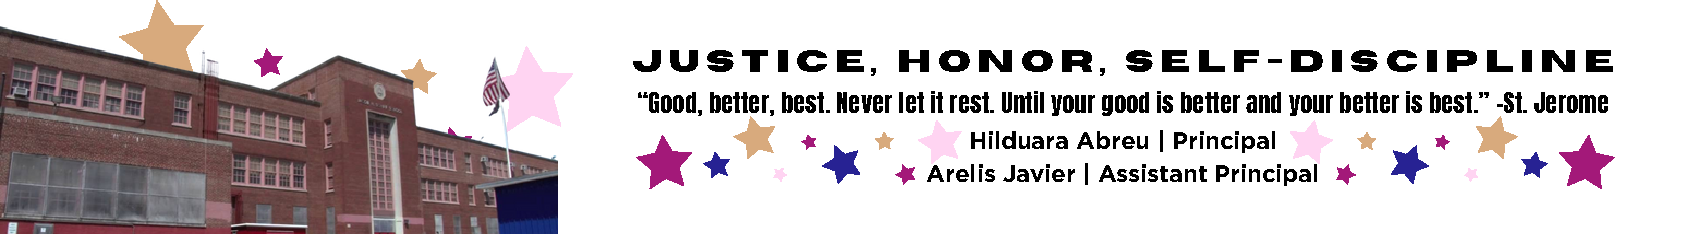
\includegraphics[width=8.8in,height=1.3in]{logo-1}}\end{picture}}
\fancyhead[C]{\setlength{\unitlength}{1in}\begin{picture}(5,0)\put(-1.9,-1){
\includegraphics[width=8.9in,height=1.3in]{logo-2}}\end{picture}}

\pagenumbering{gobble}
\addtolength{\evensidemargin}{-2in}
\addtolength{\topmargin}{-0.5in}
\addtolength{\textwidth}{0in}
%%%%%%%%%%%%%%%%%%%%%%%%%%%%%%%%%%%%%%%%%%%%%%%%%%%%%%%%%%%%%%%%%%

\begin{document}
\vspace*{0.5in}
Date: \href{https://www.ps192.org/apps/bbmessages/show_bbm.jsp?REC_ID=139439}{September 14, 2023} 

\textbf{Subject: Bell Schedule}

A bell schedule specifies the start time and duration of one or more instructional periods on each day of a day pattern. A consistent daily schedule and step-by-step
routines give children a predictable day. A Bell Schedule helps children:
\begin{itemize}
\item Feel in control of their environment
\item Feel safe, secure, and comfortable
\item Know what is happening now and what comes next
\item Know how to do an activity or task
\item Engage in learning
\end{itemize}
Just like adults, children feel more confident and secure when their daily activities are predictable and familiar.

\begin{center}
\LARGE
    \begin{tabular}{|c|c|c|c|}
    \hline
    \textbf{Description/ Period} & \textbf{Start Time} & \textbf{End Time} & 
    \textbf{Length} \\
    
    \hline
    1 & 08:00 AM & 08:45 AM & 45 minutes \\
    \hline
    2 & 08:45 AM & 09:30 AM & 45 minutes \\
    \hline
    3 & 09:30 AM & 10:15 AM & 45 minutes \\
    \hline
    4 & 10:15 AM & 11:05 AM & 50 minutes \\
    \hline
    5 & 11:05 AM & 11:55 PM & 50 minutes \\
    \hline
    6 & 11:55 PM & 12:40 PM & 45 minutes \\
    \hline
    7 & 12:40 PM & 01:30 PM & 50 minutes \\
    \hline
    8 & 01:30 PM & 02:15 PM & 45 minutes \\
    \hline
    \end{tabular}
    \end{center}



\end{document}
